\section{Результаты исследования}

В данном разделе представлены результаты анализа репрезентативности методов
формирования выборки, полученные в ходе имитационного моделирования.

% ─────────────────────────────────────────────────────────────────────────────
\subsection{Результаты разведочного анализа}

На первом этапе были рассчитаны дисперсии разведочных выборок и оценена
устойчивость выводов о лидирующем бренде. Эти показатели легли в основу
дальнейшего расчета необходимого объема целевой совокупности.

\noindent Оценки дисперсий по методам отбора:

\begin{table}[h!]
\centering
\begin{tblr}{
    colspec = {|X[l]|X[c]|},
    row{1} = {gray!30, font=\bfseries},
    row{even} = {gray!10},
    hlines,
    vlines,
}
Метод отбора & Требуемая дисперсия \\
Кластерный   & 8{,}7509   \\
Типический   & 509{,}8195 \\
Механический & 837{,}0244 \\
Случайный    & 861{,}5636 \\
\end{tblr}
\caption{Дисперсии разведочных выборок по методам}
\label{tab:pilot_variances}
\end{table}

Наименьшая дисперсия у \textit{кластерного метода} объясняется высокой
внутрикластерной однородностью: опрашиваемые на одной станции демонстрируют
схожие предпочтения, поэтому межгрупповая вариация оказывается очень мала.
\textit{Типический метод} демонстрирует выигрыш в точности по сравнению со
случайным за счет исключения межгрупповой составляющей вариации, поскольку
стратификация по поло-возрастному признаку выделяет однородные подгруппы.

% ─────────────────────────────────────────────────────────────────────────────
\subsection{Анализ устойчивости на малых выборках}

Для оценки надежности выводов на этапе разведки каждый метод запускался $100$
раз с различными зернами генератора. Подсчитывалось, сколько раз каждый из
брендов имел минимальное среднее отклонение от идеала.

\begin{table}[h!]
\centering
\begin{tblr}{
    colspec = {|X[1.2,l]|X[c]|X[c]|X[c]|},
    row{1} = {gray!30, font=\bfseries},
    row{even} = {gray!10},
    hlines,
    vlines,
}
Метод & Sony & JBL & Marshall \\
Случайный    & 42 & 42 & 16 \\
Механический & 52 & 32 & 16 \\
Типический   & 40 & 38 & 22 \\
Кластерный   & 46 & 41 & 13 \\
\end{tblr}
\caption{Частота победы каждого бренда за 100 итераций}
\label{tab:win_rates}
\end{table}

При малом объеме выборки бренды \textbf{Sony} и \textbf{JBL} статистически
неразличимы~--- при разных зернах генератора победителем может стать как первый,
так и второй. То есть победитель определяется случаным составом выборки, а 
не способом ее формирования.
Это подтверждает необходимость перехода к расчету минимально необходимого
объема выборки~($n_{min}$).

% ─────────────────────────────────────────────────────────────────────────────
\subsection{Минимальный объем выборки и точность}

Используя итерационную схему, были определены объемы выборок, обеспечивающие
заданную предельную ошибку\textsuperscript{\ref{fn:delta}}...

\begin{table}[H]
\centering
\begin{tblr}{
    colspec = {|X[l]|X[1.2,c]|X[1.2,c]|},
    row{1} = {gray!30, font=\bfseries},
    row{even} = {gray!10},
    hlines,
    vlines,
}
Метод отбора & Предельная ошибка выборки & Целевая предельная ошибка \\
Случайный    & 2{,}3534 & 1{,}1767 \\
Механический & 2{,}2728 & 1{,}1364 \\
Типический   & 1{,}8103 & 0{,}9052 \\
Кластерный   & 1{,}9873 & 0{,}9937 \\
\end{tblr}
\caption{Сравнительные показатели точности методов отбора}
\label{tab:accuracy_metrics}
\end{table}

На основе этих данных сформированы требования к объему итоговых выборок для
имитационной модели:

\begin{table}[h!]
\centering
\begin{tblr}{
    colspec = {|X[l]|X[c]|X[c]|},
    row{1} = {gray!30, font=\bfseries},
    row{even} = {gray!10},
    hlines,
    vlines,
    cell{2}{1} = {r=2}{white,l},
    cell{5}{1} = {r=2}{white!10,l},
    cell{7}{1} = {r=2}{gray!10,l},
}
Метод & Повт. & Мин. объем ($n_{min}$) \\
Случайный    & Да  & 2393 \\
             & Нет & 2064 \\
Механический & Нет & 2138 \\
Типический   & Да  & 2393 \\
             & Нет & 2064 \\
Кластерный   & Да  & 1934 \\
             & Нет & 1713 \\
\end{tblr}
\caption{Минимальный объем выборки по методам и способам отбора}
\label{tab:sample_sizes}
\end{table}

Поскольку целевая ошибка $\Delta_{GP}$\textsuperscript{\ref{fn:delta}} была задана 
относительно текущей ошибки метода, дисперсия метода математически 
сокращается (следует из формул $\eqref{eq:delta_error}, \eqref{eq:n_0}$ и $\eqref{eq:n_1}$)
при расчете первого и второго приближений минимального объема
выборки. На заданном зерне\footnote{$\texttt{SEED} = 100$} 
объемы изначальных выборок для \textit{типического} и 
\textit{случайного} методов совпали, чего могло
и не произойти. Поэтому мы наблюдаем одинаковые новые минимальные 
объемы выборок для этих двух методов.  

% ─────────────────────────────────────────────────────────────────────────────
\subsection{Имитационное моделирование}

Для каждой из семи комбинаций метода и способа отбора проводилось $10\,000$
симуляций. На каждой итерации формировалась выборка объема $n_{min}$,
вычислялись средние оценки трех брендов и фиксировался победитель.

\subsubsection{Устойчивость определения лидера}

При достижении объема $n_{min}$ неопределенность, характерная для разведочного
анализа, исчезает.

\begin{table}[h!]
\definecolor{lightgreen}{rgb}{0.85, 1, 0.85}
\definecolor{lightred}{rgb}{1, 0.85, 0.85}
\centering
\begin{tblr}{
    colspec = {|X[1.5,l]|X[0.8,c]|X[1.5,c]|X[c]|X[c]|},
    row{1} = {gray!30, font=\bfseries},
    row{even} = {gray!10},
    hlines,
    vlines,
    cell{2}{1} = {r=2}{gray!10,l},
    cell{4}{1} = {r=1}{white,l},
    cell{5}{1} = {r=2}{gray!10,l},
    cell{7}{1} = {r=2}{white,l},
    cell{4}{5} = {lightred},
    cell{7,8}{5} = {lightgreen}
}
Метод & Повт. & Объем ($n_{min}$) & Лидер & Частота побед (\%) \\
Кластерный   & Нет & 1713 & Sony & 56{,}86 \\
             & Да  & 1934 & Sony & 56{,}55 \\
Механический & Нет & 2138 & Sony & 51{,}83 \\
Случайный    & Нет & 2064 & Sony & 57{,}27 \\
             & Да  & 2393 & Sony & 57{,}05 \\
Типический   & Нет & 2064 & Sony & 58{,}40 \\
             & Да  & 2393 & Sony & 58{,}24 \\
\end{tblr}
\caption{Устойчивость выявления лидера за $10\,000$ итераций}
\label{tab:leader_stability}
\end{table}

Как видно из таблицы~\ref{tab:leader_stability}, во всех конфигурациях лидером
является \textbf{Sony}. Наиболее высокий процент побед показывает типический
метод (до~$58{,}4\%$).

\subsubsection{Усредненные оценки и вариативность}

\begin{table}[H]
\centering
\begin{tblr}{
    colspec = {|X[1.2,l]|X[c]|X[c]|X[c]|X[c]|},
    row{1} = {gray!30, font=\bfseries},
    row{even} = {gray!10},
    hlines,
    vlines,
    cell{2}{1}  = {r=6}{gray!10,l},
    cell{2}{2}  = {r=3}{c},
    cell{5}{2}  = {r=3}{c},
    cell{8}{1}  = {r=3}{white,l},
    cell{8}{2}  = {r=3}{c},
    cell{11}{1} = {r=6}{gray!10,l},
    cell{11}{2} = {r=3}{c},
    cell{14}{2} = {r=3}{c},
    cell{17}{1} = {r=6}{white,l},
    cell{17}{2} = {r=3}{c},
    cell{20}{2} = {r=3}{c},
}
Метод & Повт. & Бренд & Среднее & СКО \\
Кластерный   & Нет & Sony     & 76{,}2662 & 0{,}4445 \\
             &     & JBL      & 76{,}4096 & 0{,}3939 \\
             &     & Marshall & 76{,}9619 & 0{,}3649 \\
             & Да  & Sony     & 76{,}2605 & 0{,}4321 \\
             &     & JBL      & 76{,}4076 & 0{,}3818 \\
             &     & Marshall & 76{,}9604 & 0{,}3454 \\
Механический & Нет & Sony     & 76{,}2569 & 0{,}3322 \\
             &     & JBL      & 76{,}3946 & 0{,}2817 \\
             &     & Marshall & 76{,}9521 & 0{,}1719 \\
Случайный    & Нет & Sony     & 76{,}2622 & 0{,}3644 \\
             &     & JBL      & 76{,}3954 & 0{,}3423 \\
             &     & Marshall & 76{,}9507 & 0{,}2722 \\
             & Да  & Sony     & 76{,}2594 & 0{,}3592 \\
             &     & JBL      & 76{,}3995 & 0{,}3406 \\
             &     & Marshall & 76{,}9559 & 0{,}2711 \\
Типический   & Нет & Sony     & 76{,}2406 & 0{,}2101 \\
             &     & JBL      & 76{,}3803 & 0{,}2022 \\
             &     & Marshall & 76{,}9430 & 0{,}2040 \\
             & Да  & Sony     & 76{,}2566 & 0{,}2137 \\
             &     & JBL      & 76{,}3983 & 0{,}2048 \\
             &     & Marshall & 76{,}9531 & 0{,}2039 \\
\end{tblr}
\caption{Статистические показатели брендов по методам формирования выборки}
\label{tab:brands_tblr}
\end{table}

Все рассмотренные методы корректно воспроизводят иерархию брендов%
\footnote{\textit{Sony} $<$ \textit{JBL} $<$ \textit{Marshall}} по показателю
среднего отклонения. Это подтверждает, что качественный вывод о лидере рынка
\textit{сохраняет устойчивость вне зависимости от выбранного способа
формирования выборки}.

\subsubsection{Проверка статистической несмещенности}

Для верификации точности был применен Z-тест. Согласно описанной ранее
\hyperlink{z-test}{методике проверки статистической несмещенности}, основной
целью данного этапа является подтверждение нулевой гипотезы.

\begin{table}[h!]
\centering
\definecolor{lightgreen}{rgb}{0.85, 1, 0.85}
\definecolor{lightred}{rgb}{1, 0.85, 0.85}
\begin{tblr}{
    colspec = {|X[1.5,l]|X[0.8,c]|X[1.5,c]|X[c]|},
    row{1} = {gray!30, font=\bfseries},
    row{even} = {gray!10},
    hlines,
    vlines,
    % Логика объединения строк (ваша исходная)
    cell{2}{1} = {r=2}{gray!10,l},
    cell{4}{1} = {r=1}{white,l},
    cell{5}{1} = {r=2}{gray!10,l},
    cell{7}{1} = {r=2}{white,l},
    % ПОДЦВЕТКА ЯЧЕЕК 3/3 (Зеленый)
    cell{4,5,6,7}{3} = {lightgreen},
    % ПОДЦВЕТКА ОСТАЛЬНЫХ (Красный)
    cell{2,3,8}{3} = {lightred},
}
Метод & Повт. & Статистическая несмещенность (бренды) & Средняя дисперсия \\
Кластерный   & Да  & 2/3 & 0{,}3864 \\
             & Нет & 2/3 & 0{,}4011 \\
Механический & Нет & 3/3 & 0{,}2619 \\
Случайный    & Да  & 3/3 & 0{,}3236 \\
             & Нет & 3/3 & 0{,}3263 \\
Типический   & Да  & 3/3 & 0{,}2075 \\
             & Нет & 1/3 & 0{,}2055 \\
\end{tblr}
\caption{Результаты проверки точности и надежности методов формирования выборки}
\label{tab:accuracy_reliability}
\end{table}

Несмотря на минимальную дисперсию ($0{,}2055$) у \textit{повторного типического} метода отбора, он обеспечивает несмещенность лишь для одного из трех брендов. Это объясняется тем, что при
большом~$n_{min}$ и фиксированном объеме страт бесповторный отбор фактически
исчерпывает часть страт, нарушая случайность и внося систематическое
отклонение. \textit{Кластерный} метод демонстрирует аналогичную структурную проблему
независимо от режима повторности~--- следствие внутрикластерной
однородности по предпочтениям к отдельным брендам.

Оптимальным по совокупности критериев является \textbf{типический повторный}
метод: он единственный достигает полной несмещенности (3/3) при наименьшей
дисперсии среди несмещенных методов ($0{,}2075$).

\clearpage

% ─────────────────────────────────────────────────────────────────────────────
\subsection{Визуализация и интерпретация}

Для итогового сравнения надежности методов построена столбчатая диаграмма
дисперсии оценок по каждому бренду в разбивке по методу и способу отбора
(рис.~\ref{fig:variance_plot}).

\begin{figure}[h!]
    \centering
    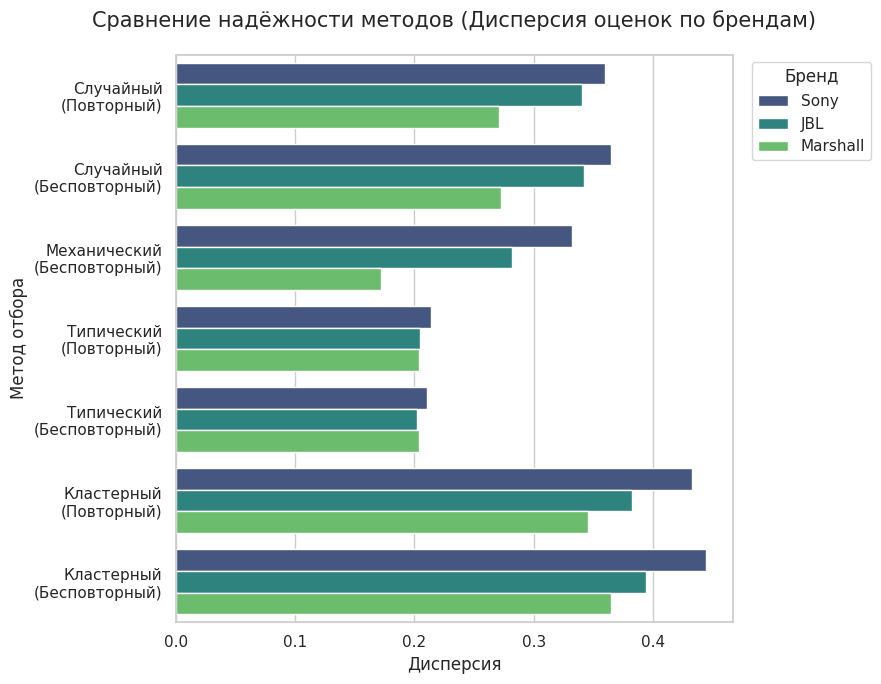
\includegraphics[width=\linewidth]{images/output.png}
    \caption{Сравнение надежности методов: дисперсия оценок по брендам}
    \label{fig:variance_plot}
\end{figure}

\textbf{Случайный метод} служит базовым ориентиром для сравнения: не используя
никакой информации о структуре совокупности, он демонстрирует наибольшую
дисперсию среди несмещённых методов. Повторный и бесповторный режимы
дают практически идентичные результаты~--- при $n \ll N$ поправка на
бесповторность пренебрежимо мала. Повышенная дисперсия для Sony и JBL
относительно Marshall свидетельствует о неоднородности предпочтений
респондентов к этим брендам, которую случайный отбор не способен
контролировать.

На диаграмме четко прослеживается превосходство \textbf{типического отбора}:
он обеспечивает минимальный разброс оценок для всех трех брендов, что делает
его наиболее предпочтительным для маркетинговых исследований в условиях
известной структуры совокупности. 

\textbf{Кластерный} метод уступает всем остальным по стабильности оценок:
высокая дисперсия отражает сильную зависимость результата от того, какие
именно кластеры попали в выборку.

Аномально низкая дисперсия \textbf{механического метода} для бренда Marshall, возможно, вызван равномерным распределением оценок этого бренда вдоль
отсортированного датасета: при фиксированном шаге $k$ любая стартовая
позиция захватывает репрезентативное подмножество.
